\section{Conclusion}
\label{ch:conclusion}

With our new cheat detection system we hope that gaming has forever been changed for the better. The competitive integrity and player enjoyment ruined by cheating may not have been completely eradicated but our findings and results have reduced it by a significant amount. 

We hope that our research proves useful for the gaming industry as our results have shown that we have a greatly improved chance against cheating. Our findings have not only increased the success rate of cheat detection but also gave a more reliable and explainable way of examining players' actions and their behaviours while preventing them from cheating and ruining other users' enjoyment of games.

The anti-cheat model we implemented created a more reliable competitive space in gaming and a scarier and more effective guard against cheaters. The results showed that creating a cheat-free environment increased player enjoyment and user numbers in video games.

Our research showed that the use of AI is indeed a viable and incredibely useful tool for cheat detection in gaming. We think this research is evidence that the use of AI is a must for keeping games clean from cheaters and keeping the competitive integrity of games.

\begin{figure}[h]
\centering
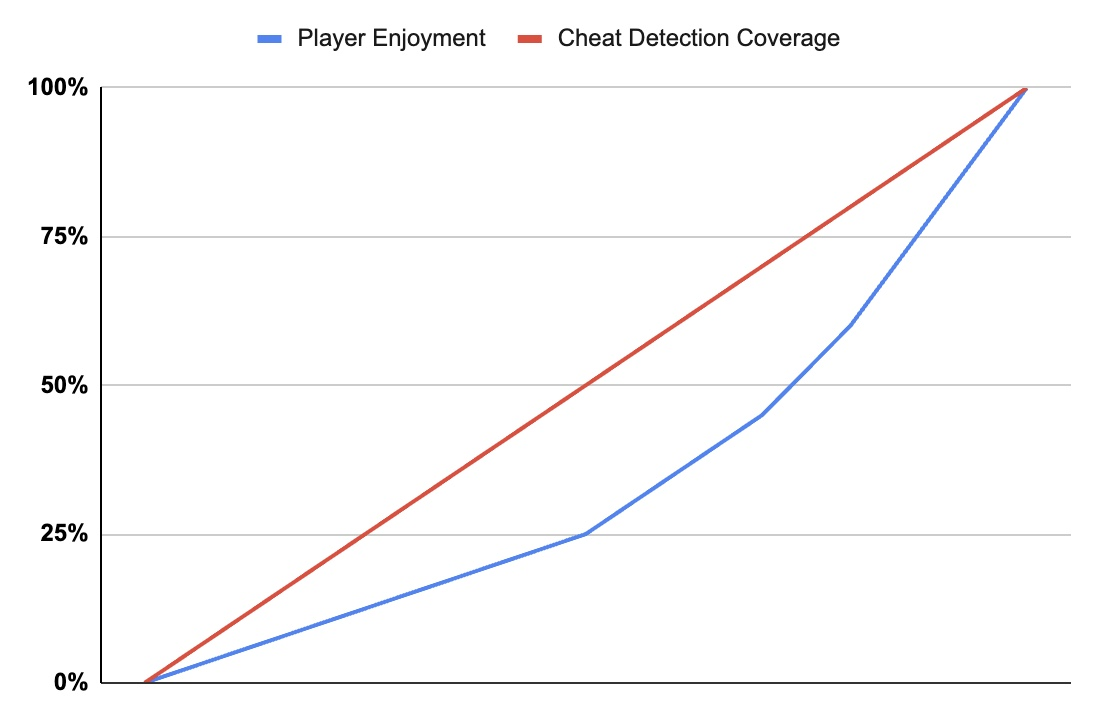
\includegraphics[width=0.6\linewidth]{images/enjoyment.jpeg}
\captionsetup{width=0.6\textwidth}
\caption{\label{fig:enjoyment}Graph showing the correlation between player enjoyment and cheat detection coverage.}
\end{figure}